\qrchapter{https://forgottenpillar.com/rsc/hr-fp-chapter12}{Realnost Neba}

\emcap{Ličnost Boga} se bavi kvalitetom ili stanjem koja Boga čine osobom. Kad god pogledamo spise pionira o \emcap{ličnosti Boga}, vidimo da su svi bili u skladu s pogledom da je Bog opipljivo \textit{biće}, koje posjeduje i tijelo i dijelove. Uvijek vidimo isto temeljno rasuđivanje, koje razlikuje pojam ‘\textit{duh}’ i pojam ‘\textit{biće}’. Razlikujući ove pojmove, oni objašnjavaju kvalitetu ili stanje koja Boga čine osobom\footnote{\href{https://www.merriam-webster.com/dictionary/personality}{Merriam-Webster Dictionary} definira riječ ‘\textit{personality}’ kao “\textit{kvaliteta ili stanje koja nekog čine osobom}”.}—\emcap{ličnost Boga}. Svi njihovi zaključci su sažeti u prvoj točki \emcap{Fundamentalnih Principa}. \others{Postoji \textbf{jedan Bog}, \textbf{osobno}, \textbf{duhovno biće}, Stvoritelj svega, svemoguć, sveznajući, … i \textbf{svugdje prisutan preko svog predstavnika, Svetog Duha}. Psalam 139:7.}[FPSDA 1.2][https://egwwritings.org/read?panels=p1299.6]

Dosad smo u spisima pionira vidjeli da je \emcap{ličnost Boga} usko povezana s realnošću Božje prisutnosti. Bog je osobno duhovno biće, ima tijelo i oblik; te kao takav, Njegova prisutnost je ograničena na jedan lokalitet—kako Biblija kaže, u Njegovom hramu, na Njegovom prijestolju gdje je okružen nepristupačnom slavom. No, On je svuda prisutan preko Svog predstavnika, Svetog Duha. Očito, Sveti Duh je duh, a ne biće, \bible{duh nema tijela i kostiju kao što vidite da ja imam}, rekao je Isus (Luka 24:39). Krist je također Biće, kao i Njegov Otac. On je savršena slika Očeve osobe; stoga nosi jednaku ličnost, ili kvalitetu ili stanje koja ga čine osobom, baš kao i Njegovog Oca.

U našem iskustvu, kada bismo predstavili našoj trinitarnoj braći originalna vjerovanja Adventista Sedmog Dana o \emcap{ličnosti Boga}, kako je izraženo u prve dvije točke \emcap{Fundamentalnih Principa}, često su tvrdili kako su izjave u \emcap{Fundamentalnim Principima} na neki način točne, ali da je razumijevanje pripisano terminima “\textit{osobno duhovno biće}” pogrešno. Obično pokušavaju uskladiti \emcap{Fundamentalne Principe} s doktrinom o Trojstvu izvrćući riječi “\textit{duhovno biće}”, kao da riječ ‘\textit{duhovno}’ znači nešto tajanstveno, prikladno da izjednači \emcap{ličnost Boga} i Krista s ličnošću Svetog Duha\footnote{Kvaliteta ili stanje koje Duha Svetoga čini osobom jest svjedočenje, a ne posjedovanje oblika osobe. \egw{\textbf{Duh Sveti ima osobnost}, \textbf{\underline{inače} ne bi mogao \underline{svjedočiti} našem duhu} i s našim duhom da smo djeca Božja. \textbf{On također mora biti božanska osoba}, \textbf{\underline{inače} ne bi mogao \underline{istražiti} tajne koje leže skrivene u umu Božjem}. ‘Jer tko od ljudi zna što je u čovjeku osim duha čovječjega u njemu? Tako i što je u Bogu, nitko ne zna osim Duha Božjega.’ [1 Korinćanima 2:11.]}[21LtMs, Ms 20, 1906, par. 32][https://egwwritings.org/read?panels=p14071.10296041&index=0]. Kristalno je jasno da je Duh Sveti osoba, ali ne na isti način kao Otac i Sin, jer Duh Sveti ne posjeduje kvalitetu vanjske fizičke ličnosti kao što to imaju Otac i Sin.}. Temeljni problem svodi se na razumijevanje nebeskih stvarnosti. Biblija ne šuti o nebu i njegovim stvarnostima, i naši pioniri su to dobro shvatili. Ispod čitamo o objašnjenju termina “\textit{duhovno biće}” iz knjige Jamesa Whitea i Uriaha Smitha, “\textit{Biblijski Institut}”. Biblija objašnjava te termine koristeći primjer anđela, koji su “\textit{duhovna bića}”.

\begin{figure}[hp]
    \centering
    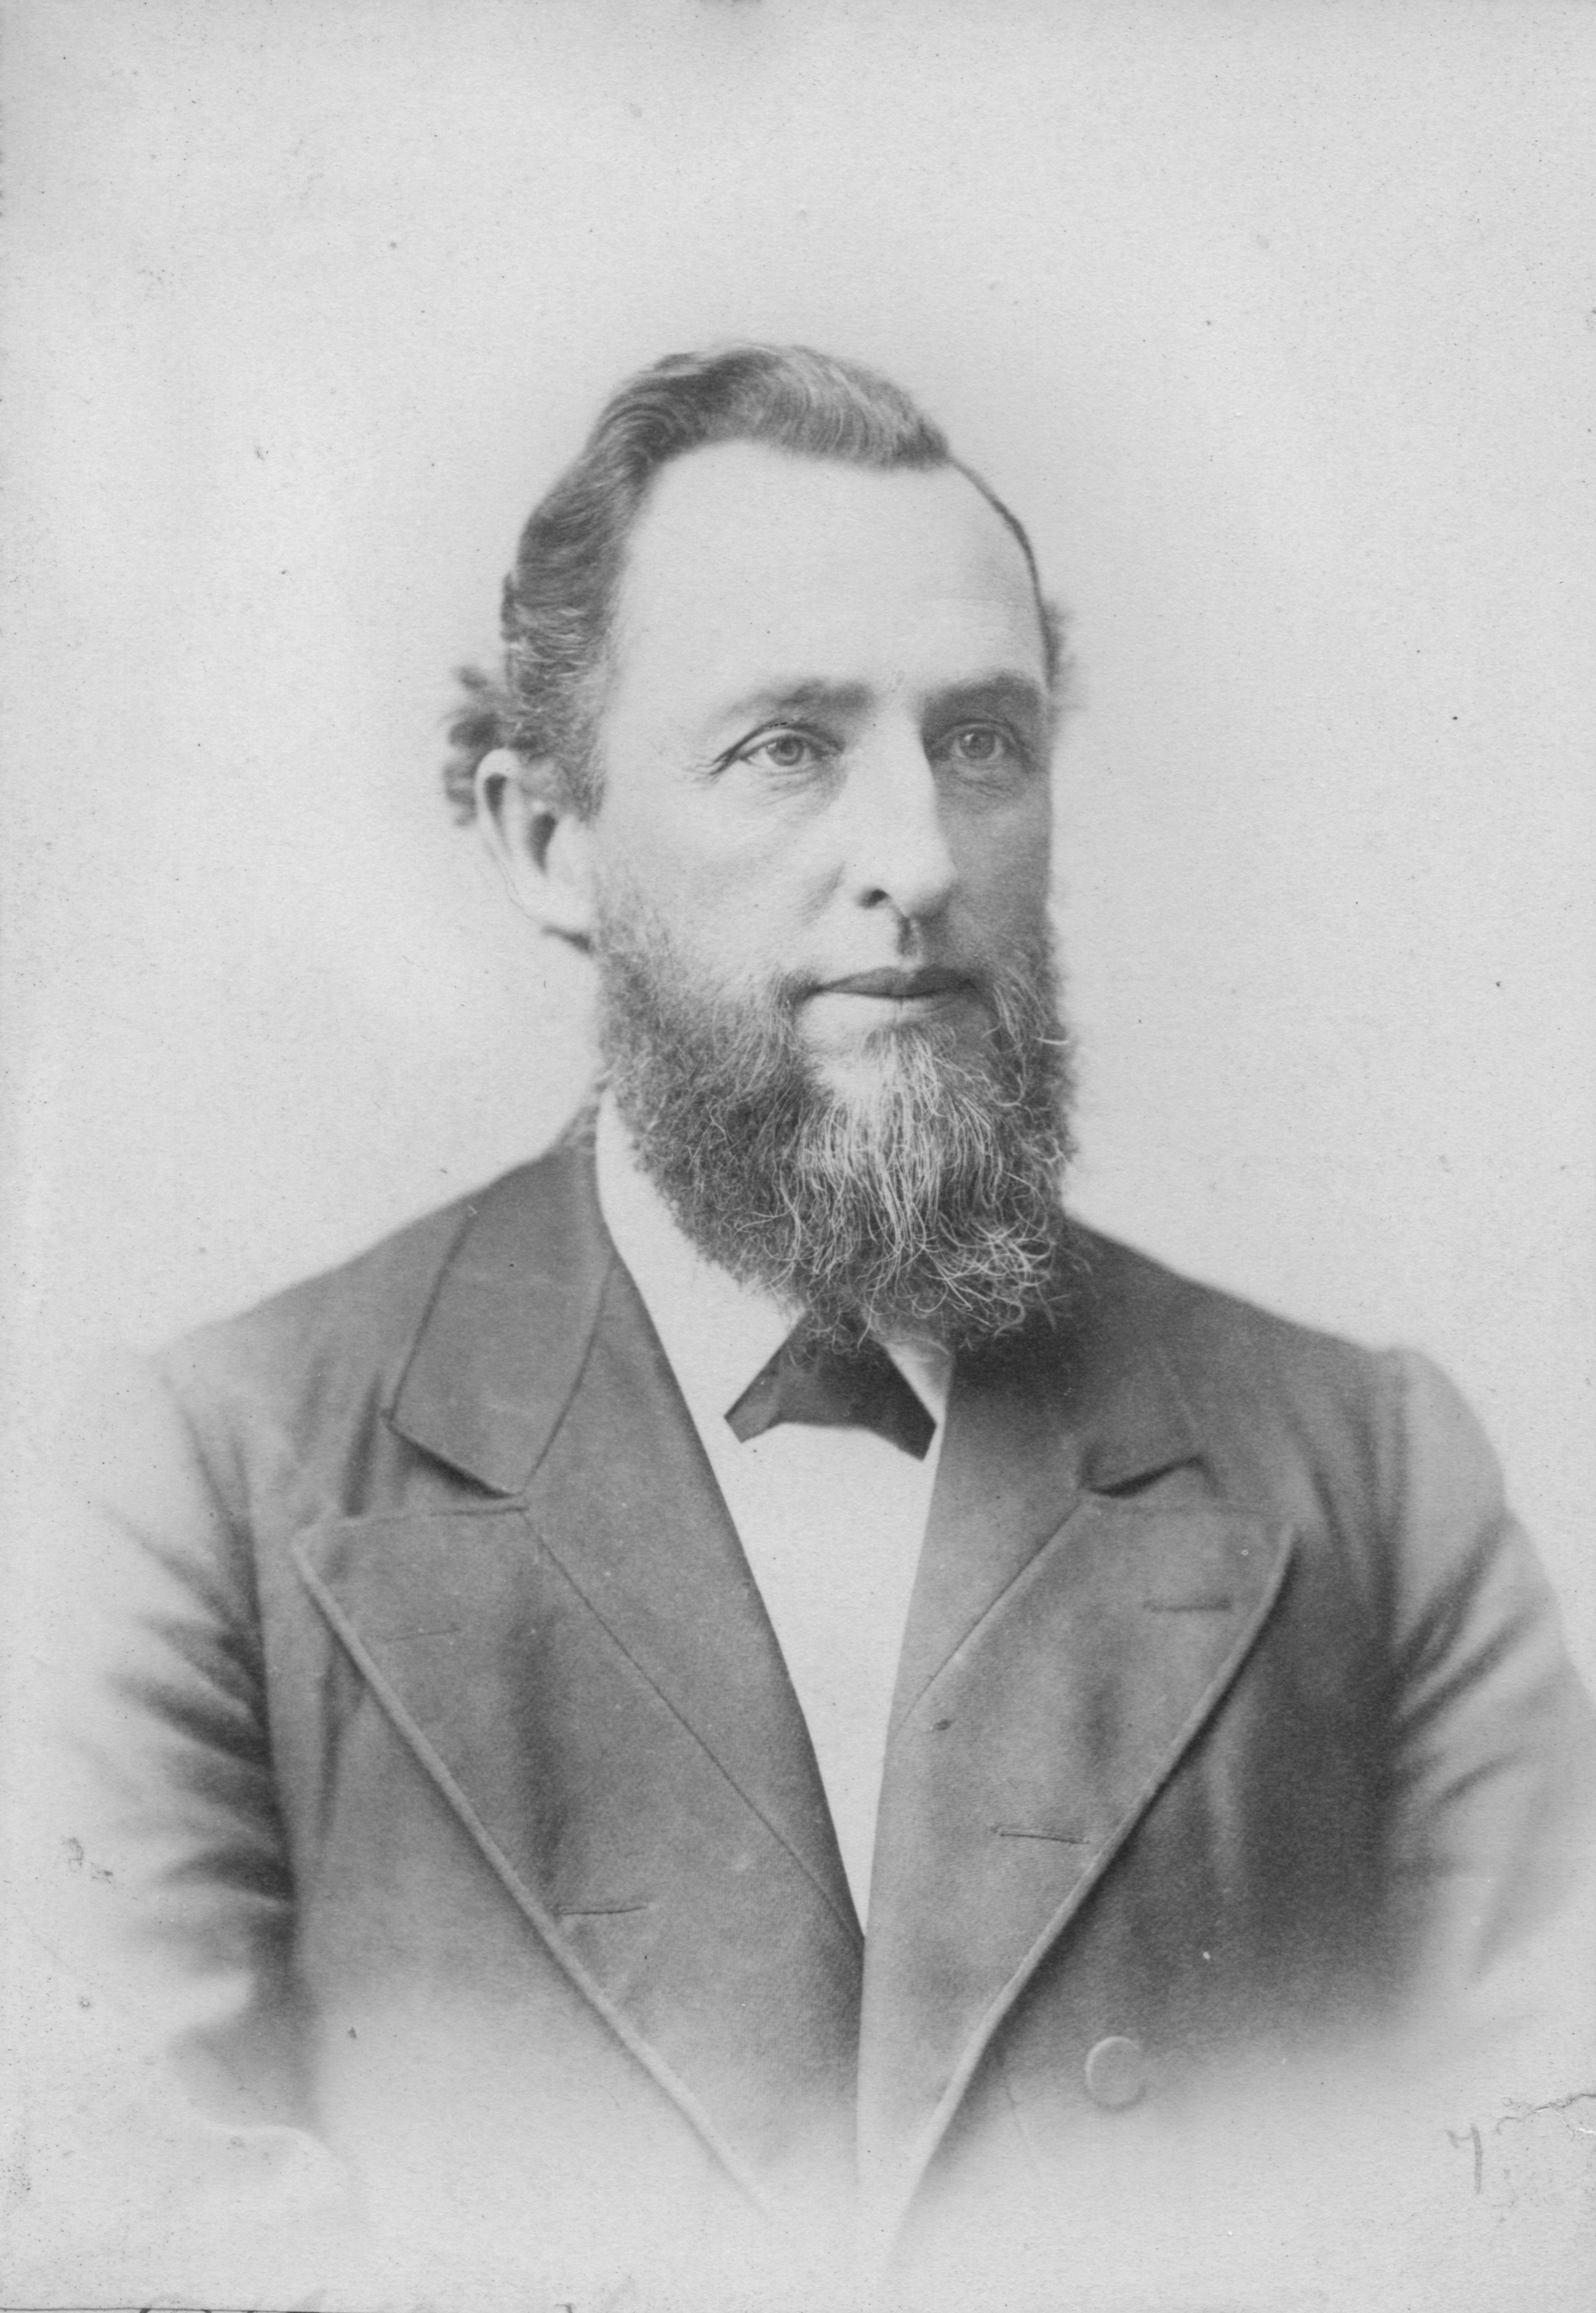
\includegraphics[width=1\linewidth]{images/uriah-smith.jpg}
    \caption*{Uriah Smith (1832-1903)}
    \label{fig:uriah-smith}
\end{figure}

\others{\textbf{Anđeli su stvarna bića}. U Bibliji su opisani kao oni koji \textbf{posjeduju lice, stopala, krila} itd. Ezekiel kaže za kerubine, ‘\textbf{A cijelo njihovo \underline{tijelo} i leđa njihova i ruke njihove i krila njihova},’ itd. Eze. 10:12. Anđeli su se \textbf{ukazali} Abrahamu. Post. 18:1-8. Razgovarali su i jeli s njim. Otišli su u Sodomu i razgovarali s Lotom, koji je, ušavši u svoju kuću, ispekao beskvasni kruh za njih i oni su jeli. \textbf{Ove osobe su nazivane anđelima}. David govori o mani kao o nebeskom žitu i anđeoskoj hrani. Ps. 78:23-25.}

\othersnogap{Bileamov slučaj, Br. 22:22-31, zanimljiv je događaj. Anđeo se \textbf{ukazao} Bileamu s \textbf{isukanim mačem u ruci}. Ponekad se postavlja pitanje \textbf{kako anđeli mogu biti \underline{materijalna bića kad ih ne možemo vidjeti}. Ovaj slučaj to ilustrira}. Zapis kaže da je \textbf{Gospodin otvorio oči Bileamu i on je ugledao anđela}. \textbf{Anđeo nije stvorio tijelo za tu priliku}. \textbf{Bio je isti kakav je bio prije nego što ga je Bileam ugledao; ali se \underline{promjena dogodila u Bileamu}}. Oči su mu se otvorile, a zatim je ugledao anđela. Isto je bilo s Elizejevim slugom kad su on i njegov gospodar bili dovedeni u dolinu, okruženi vojskom sirijskog kralja. 2. Kraljevima 6:17. Elizej se molio da se \textbf{oči njegova sluge otvore}; i odmah ugleda cijelu planinu punu konja i bojnih kola oko Elizeja.}

\othersnogap{\textbf{Ovo se može dodatno ilustrirati pozivajući se na stvari za koje znamo da su materijalne, a koje ipak ne možemo vidjeti}. Zrak je materijal, svjetlost je materijalna, čak je i sama misao samo rezultat materijalnih organizacija—materija djeluje na materiju—a ipak ne možemo vidjeti ništa od toga. \textbf{Tako je i s anđelima}.}

\othersnogap{\textbf{Nadalje, prigovor za materijalnost anđela je da se nazivaju duhovima}. Hebr. 1:13, 14. \textbf{\underline{Ali to nije prigovor da su oni doslovna bića}}. \textbf{Oni su jednostavno duhovna bića organizirana drugačije od ovih zemaljskih tijela koja posjedujemo}. Pavao kaže, 1 Kor. 15:44, ‘\textbf{Postoji prirodno tijelo i postoji \underline{duhovno tijelo}}.’ \textbf{Prirodno tijelo koje sada imamo; duhovno tijelo koje ćemo imati u uskrsnuću}. ‘\textbf{Ustaje duhovno tijelo}.’ Stih 44. \textbf{Ali tada smo jednaki anđelima}, Luka 20:36; \textbf{tada imamo tijela slična Kristovom najslavnijem tijelu}. Fil. 3:4 \textbf{a Krist nije ništa manje duh od anđela}. \textbf{Čitamo da je Bog duh, to jest jednostavno \underline{duhovno biće}}.}[James White and Uriah Smith, The Biblical Institute (Kindle Lokacija 2537-2553). Kindle Verzija.]

Biblija nam daje uvid da su anđeli duhovna bića koja posjeduju materijalna tijela, ali su nam i dalje nevidljiva, osim ako Gospodin ne otvori naše oči da ih vidimo. Kada pravednici uskrsnu u svojim novim proslavljenim tijelima, uskrsnut će u duhovnom tijelu, nepropadljivom. To tijelo će biti opipljivo i materijalno, baš kao što će Nova Zemlja biti opipljiva i materijalna. I s našim duhovnim tijelima posjedovat ćemo obnovljenu Zemlju: \bible{plodite se i množite i napunite zemlju, i sebi je podložite! I budite gospodari ribama morskim i pticama nebeskim i svemu živomu što gmiže po zemlji!}[Postanak 1:28].

% Stvarnost Neba

\begin{titledpoem}
    \stanza{
        Bog nije tajna ni nestvarna sila, \\
        Već biće stvarno što nebo je svila. \\
        Tijelo i oblik On zaista ima, \\
        Na prijestolju sjedi, vidljiv anđelima.
    }

    \stanza{
        Duhovno biće, ali ipak stvarno, \\
        Prisutan svugdje, ali ne proizvoljno. \\
        Kroz Svetoga Duha svugdje djeluje, \\
        Predstavnik Njegov svijetom putuje.
    }

    \stanza{
        Sin slika Oca, iste naravi, \\
        Obojica bića u stvarnoj pojavi. \\
        Anđeli također tijela imaju, \\
        Iako se našim očima ne daju.
    }

    \stanza{
        U uskrsnuću i mi ćemo biti, \\
        Poput anđela, duhovna tijela zadobiti. \\
        Tijela duhovna, ali opipljiva, \\
        Na Zemlji novoj, stvarnoj i predivnoj.
    }
\end{titledpoem}

